%!TEX root = ../dokumentation.tex

\chapter{Robotersteuerung und -Programmierung}
Bei dieser Studienarbeit wurde ein ABB-Industrieroboter vom Typ \enquote{IRB 140} eingesetzt. Dieser wird gesteuert über eine \enquote{IRC 5 Einzelschrank-Steuerung}. Die besteht aus folgenden Modulen: (\cite{irc5} S.7)

\begin{itemize}
\item Antriebsmodul, in dem sich das Antriebssystem befindet.

\item Steuerungsmodul, das den Computer, den Netzschalter, Kommunikationsschnittstellen und den FlexPendant-Anschluss enthält. Die Steuerung enthält auch die Systemsoftware (RobotWare-OS), welche alle grundlegenden Funktionen für Betrieb und Programmierung umfasst.
\end{itemize}

Sämtliche Operationen und Programmierungen können mithilfe des portablen FlexPendant und über RobotStudio extern ausgeführt werden. 

RobotStudio ist eine Software von ABB, die dafür gedacht ist ganze Arbeitsstationen von Industrierobotern virtuell zu erstellen, um daran dann Programme für diese Roboter entwickeln und simulieren zu können, bevor sie auf den Roboter aufgespielt werden. Die Funktionalitäten dieser Software sind sehr umfangreich und deren Beschreibung würde den Rahmen dieser Studienarbeit bei weitem sprengen. Alle Funktionalitäten, die wir genutzt haben und die man benötigt um das Projekt fortzuführen, werden in Kapitel~\ref{manual} ab Seite~\pageref{manual} beschrieben. 

Möchte man sich in die Benutzung dieser Software einarbeiten, findet man auf der Seite \href{http://new.abb.com/products/robotics/robotstudio/how-to-use-it/getting-started}{http://new.abb.com/products/robotics/robotstudio/how-to-use-it/getting-started} gute verständliche Tutorials für Einsteiger. Weiterführende Tutorials findet man auf der Seite \href{http://new.abb.com/products/robotics/robotstudio/tutorials}{http://new.abb.com/products/robotics/robotstudio/tutorials}.

Wie man den Roboter über das FlexPendant steuern kann, wird in Abschnitt \ref{flexsection} beschrieben.

Zur Programmierung steht die Hochsprache RAPID zur Verfügung, die speziell für die Steuerung von Industrierobotern von ABB entwickelt wurde. Die Datentypen und Funktionen, die nötig sind um damit eine Bewegungen des Roboterarms zu realisieren, sind in Abschnitt~\ref{rapidsection} beschrieben.

\section{Robotersteuerung mit dem FlexPendant}
\label{flexsection}
\begin{wrapfigure}{l}{.4\textwidth}
\centering
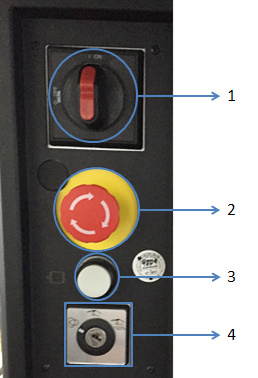
\includegraphics[height=.45\textwidth]{schaltschrank.PNG}
\vspace{-15pt}
\caption{Schaltschrank} 
\label{schaltschrank}
\end{wrapfigure}

Um den Roboter über das FlexPendant bedienen zu können, muss man zunächst den Betriebsartenwahlschalter (Schalter 4 in Abb.~\ref{schaltschrank}) auf Handbetrieb stellen. Dafür benötigt man den Schlüssel mit der Aufschrift \enquote{Schaltschrank Roboter 1}. Für den Handbetrieb gibt es zwei Modi: Schlüssel auf die rechte Position (\enquote{Handbetrieb 100\%}) bedeutet, der Roboter bewegt sich mit voller Geschwindigkeit. Schlüssel in mittlerer Position bedeutet, dass sich der Roboter mit einer reduzierten Geschwindigkeit von maximal 250 mm/s fortbewegt.

Über das FlexPendant kann der Roboter dann entweder über den Joystick (Schalter A in Abb.~\ref{flexpendant}) ferngesteuert werden, oder es können Programme ausgeführt werden, die sich auf dem Controller befinden. Dabei muss man jedoch beachten, dass immer der sogenannten \enquote{Totmannschalter} betätigt wird, welcher sich seitlich rechts am FlexPendant befindet. Dieser darf nicht zu schwach und nicht zu stark gedrückt werden und soll damit gewährleisten, dass bei einem Unfall der Roboter sofort stehen bleibt. Ob er richtig betätigt wurde erkennt man, wenn Schalter 3 am Schaltschrank (siehe Abb.~\ref{schaltschrank}) durchgängig leuchtet. 

\subsection{Fernsteuerung des Roboters}

\begin{figure}[htbp]
\centering
\includegraphics[width=10cm]{Flexpendant.png}
\caption{FlexPendant} 
\label{flexpendant}
\end{figure}

Möchte man den Roboter über den Joystick fernsteuern, so muss man zunächst in der oberen linken Ecke des Touchscreens auf das ABB-Logo klicken und anschließend auf \enquote{Bewegen}. Der Roboterarm kann auf zwei verschieden Arten bewegt werden:

\begin{enumerate}
\item Möchte man das Werkzeug linear entlang der drei Raumachsen bewegen, so muss man Knopf B auf dem FlexPendant (siehe Abb. ~\ref{flexpendant}) betätigen. Es werden dabei die entsprechenden kartesischen Koordinaten angezeigt, je nachdem welches Werkobjekt man auswählt hat. Diese Positionsangaben beziehen sich auf den Arbeitspunkt des angegebenen Werkzeugs. Ist dies \enquote{tool0} so bezieht sich diese Angabe auf den Mittelpunkt des Werkzeughalters. Zusätzlich wird auch die Orientierung des Werkzeughalters (als Quaternion\footnote{Quaternionen sind eine Erweiterung der reellen Zahlen auf vier Dimensionen ähnlich den komplexen Zahlen. Sie  sind  sehr  vielfältig  einsetzbar, beispielsweise könne sie auch zur Beschreibung von Orientierungen im Raum genutzt werden \cite{quaternion}.} ausgedrückt) angezeigt. 

\item Es ist auch möglich jede des sechs Achsen einzeln anzusteuern. Um die ersten drei Achsen anzusteuern muss man Knopf C auf dem FlexPendant (siehe Abb. ~\ref{flexpendant}) betätigen. Möchte man die Achsen vier bis sechs bewegen, einfach Knopf C erneut betätigen. 
\end{enumerate}

\subsection{Programm starten}

Möchte man über das FlexPendant ein RAPID-Programm auf dem Controller starten, so muss man zunächst in der oberen linken Ecke des Touchscreens auf das ABB-Logo klicken und anschließend auf \enquote{Programm Editor}. Hier kann man nun neue Programme schreiben oder bereits vorhandene editieren. Möchte man ein Programm starten, muss man in der unteren Leiste auf den Touchscreen auf \enquote{Testen} klicken. Nun kann man noch den Programmzähler an die gewünscht Stelle setzen: An den Anfang des Programms mit \enquote{PZ~$--$> main}, oder zu einem Unterprogramm \enquote{PZ~$--$> Routine ...}, oder an die Stelle an der sich der Cursor gerade befindet \enquote{PZ~$--$> Cursor}. Zum Starten dann auf \enquote{Play} drücken (siehe Abb.~\ref{flexpendant} Bereich D). Mit den Pfeiltasten in Bereich D kann man das Programm auch schrittweise vorwärts bzw. rückwärts ablaufen lassen.

\section{Einführung in RAPID}
\label{rapidsection}

RAPID ist eine Programmiersprache, die von ABB eigens für die Programmierung von Industrierobotern entwickelt wurde. Dabei handelt es sich um eine höhere Programmiersprache. Sie umfasst den Großteil der Funktionalitäten anderer höherer Programmiersprachen (bedingte Anweisungen, verschiedene Schleifen, so wie zahlreiche Funktionen und Datentypen). Des weiteren enthält RAPID jedoch Instruktionen zum Bewegen des Roboters.

In diesem Abschnitt werden nur die wichtigsten Datentypen und Funktionen beschrieben, die benötigt werden um den Roboterarm bewegen zu können. 

Möchte man sich mit dieser Programmiersprache vertraut machen, sollte man sich zunächst Dokument\cite{rapid1} anschauen. Eine vollständig Auflistung und Beschreibung aller Funktion, Instruktionen und Datentypen findet man im Referenzhandbuch\cite{rapid2}.

\subsection{Positionen angeben}
\label{ropbtargetsection}
Zur Definition von Positionsdaten gibt es in RAPID den Datentyp \enquote{robtarget}. Dieser Datentyp ist ein Array aus vier Komponenten:
\begin{enumerate}
\item \textbf{Translation:}

Ein dreistelliges Tupel, mit dem die Postion (x,y,und z) des Werkzeugarbeitspunkts in Millimeter angegeben wird.
\item \textbf{Rotation:}

Ein vierstelliges Tupel mit dem die Orientierung des Werkzeugs mit Quaternionen angegeben wird.

\item \textbf{Roboter Konfiguration:}

Ein vierstelliges Tupel mit dem die Achsenkonfiguration des Roboters (cf1, cf4, cf6 und cfx) angegeben wird. Diese wird als Viertelumdrehung von Achse 1 (cf1), Achse 4 (cf4) und Achse 6 (cf6) definiert. Die erste positive Viertelumdrehung (0$ ^\circ $ - 90$ ^\circ $) der drei Achsen wird dabei zum Beispiel mit 0 definiert. Mit cfx wird eine der acht möglichen Roboterkonfigurationen gewählt, die von 0 bis 7 nummeriert sind. Diese legen fest, wie die Roboterposition in Relation zu den drei Singularitäten stehen. Abbildung ~\ref{achsenkonfi} zeigt an zwei Beispielen, wie sich unterschiedliche Werte auswirken können.  
\item \textbf{Externe Achsen:}

Es ist möglich bis zu sechs weitere externe Achsen zu berücksichtigen. Hat man keine externen Achsen, muss man hier für alle sechs Werte \enquote{9E9} einsetzen. 
\end{enumerate} 

Dabei ist zu beachten, dass die Translations- und Rotations-Koordinaten sich immer auf das aktuelle Objekt-Koordinatensystem beziehen. Ist kein Werkobjekt angegeben, ist dies das Weltkoordinatensystem. 

\pagebreak
Die Definition einer Positions-Variablen könnte damit beispielsweise lauten:

\begin{lstlisting}[caption=Beispiel für die Definition einer Position, label=robtarget, language=bash]
CONST robtarget Target_1:=[[453,26,610],[1,0,0,0],[-1,0,0,0],[9E9,9E9,9E9,9E9,9E9,9E9]];
\end{lstlisting} 

\begin{figure}[htbp]
\centering
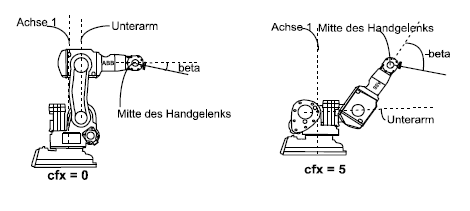
\includegraphics[width=12cm]{achsenkonfi.png}
\caption{Achsenkonfigurationen für cfx = 0 und cfx =5 (\cite{rapid2} S. 1160ff)} 
\label{achsenkonfi}
\end{figure}

\subsection{Pfade abfahren}
\label{movesection}
Zum Bewegen des Roboters bietet die Programmiersprache RAPID zahlreiche Möglichkeiten. So kann man beispielsweise mit MoveAbsJ-Instruktion jede Achse einzeln ansteuern, indem man dem Roboter eine absolte Achsenposition übergibt. Zur Realisierung einer Kreisbewegung kann MoveC verwendet werden. MoveJ wird verwendet, um den Roboter rasch von einem Punkt an einen anderen zu bewegen, wenn diese Bewegung nicht geradlinig sein muss. In diesem Projekt sollte dies aber gerade der Fall sein. Zur Ansteuerung des Roboters wurde deshalb ausschließlich die Instruktion MoveL genutzt, mit der sich lineare Bewegungen realisieren lassen. 

Die Instruktion MoveL erwartet mindestens vier Pflicht-Übergabeparameter, außerdem können ihr noch acht weitere optionale Parameter übergeben werden. Im folgenden werden die vier Pflichtkomponenten und die beiden wichtigsten optionalen Komponenten beschrieben.

%rapid1 S.25 und rapid2 S.280 
\begin{enumerate}
\item \textbf{Zielpunkt:}

Eine Variable vom Typ \enquote{robtarget} (siehe ~\ref{ropbtargetsection}).
\item \textbf{Geschwindigkeit:}

Parameter von Datentyp \enquote{speeddata}, der die Geschwindigkeit des Werzeugarbeitspunktes, der Werkzeugumorientierung und der externen Achsen definiert. Im System-Module \enquote{BASE} auf dem Roboter-Controller findet man bereits vordefinierte Variablen dieses Typs. Übergibt man beispielsweise die Variable \enquote{v1000}, soll sich der Roboter mit einer Geschwindigkeit von 1000 mm/s bewegen. 
\item \textbf{Zone:}

Variable vom Typ \enquote{zonedata}, die angibt wie nahe sich der Werkzeugarbeitspunkt an der angegeben Zielposition befinden muss, bevor der Roboter an die nächste Position bewegt werden kann. Auch hierfür sind im System-Modul \enquote{BASE} bereits Variablen vordefiniert. In diesem Projekt sollte immer die übergebene Position erreicht werden. Dies kann man durch Übergabe der vordefinierten Variable \enquote{fine} erreicht werden. Verwendet man stattdessen beispielsweise \enquote{z10}, bedeutet dies, dass der Roboter die Ecken schneiden kann, sobald er weniger als 10 mm von der Zielposition entfernt ist.
\item \textbf{Werkzeug:}

Angabe, welches Werkzeug am Roboter montiert wird. Dessen Arbeitspunkt wird dann zur angegebenen Position bewegt. In diesem Projekt wurde hier immer \enquote{tool0} verwendet. D.h. es wird immer der Mittelpunkt des Montageflansches an der Spitze des Roboters an die übergebene Position bewegt.\footnote{Dies kann man nur machen, wenn der Roboter ausschließlich linear bewegt wird und somit der Arbeitspunkt des Werkzeugs immer um den gleichen Vektor zum Mittelpunkt des Montageflansches verschoben ist.}  
\item \textbf{Werkobjekt:}

Dies ist ein optionaler Übergabeparameter vom Typ \enquote{wobjdata}. Er gibt an auf welches Koordinatensystem sich die Roboterposition in der Instruktion bezieht. Übergibt man kein Werkobjekt wird das Weltkoordinatensystem verwendet. 
\item \textbf{Zeit:}

Dies ist ein optionaler Übergabeparameter vom Typ \enquote{num}. Also einfach ein Zahlenwert, der die Gesamtdauer, die der Roboter für die Bewegung benötigen soll,  in Sekunden angibt. Dieser Wert ersetzt dann die entsprechenden Geschwindigkeitsdaten.
\end{enumerate}

Der Aufruf einer MoveL-Instruktion könnte dann beispielsweise lauten:

\begin{lstlisting}[caption=Beispielaufruf der MoveL-Instruktion, label=movel, language=bash]
MoveL Target_1,v500,fine,tool0 \WObj:=Workobject_Table;
\end{lstlisting}